% Propósito: integrar las pistas físicas y perceptuales que intervienen al
% seleccionar una voz entre fuentes concurrentes, evitando representar el
% efecto cocktail party como un filtro físico único.
% Origen: factores enumerados en la sección
% \ref{sec:u7-cocktail-party}. Escena conceptual sin datos ni resultado
% clínico.
% Descripción accesible: una persona escucha una voz objetivo situada al
% frente, dos voces competidoras a los lados y ruido de ventilación detrás. Las
% flechas llegan a ambos oídos. Un bloque lateral separa pistas físicas como
% SNR y dirección de procesos perceptuales como segregación y atención.
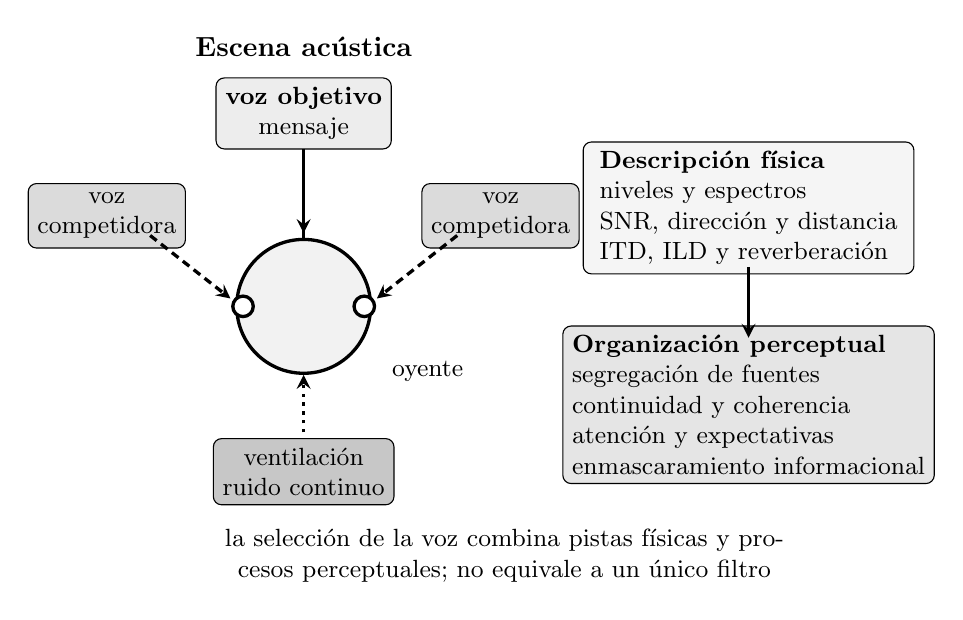
\begin{tikzpicture}[font=\small,>=stealth,x=1cm,y=1cm]
    \node[font=\bfseries] at (3.45,5.85)
        {Escena acústica};

    \draw[very thick,fill=black!5] (3.45,2.55) circle (0.85);
    \draw[very thick,fill=white] (2.68,2.55) circle (0.13);
    \draw[very thick,fill=white] (4.22,2.55) circle (0.13);
    \draw[very thick] (3.45,3.40) -- (3.45,3.82);
    \node[anchor=west] at (4.45,1.72) {oyente};

    \node[draw,rounded corners=3pt,fill=black!7,align=center] at (3.45,5.00)
        {\textbf{voz objetivo}\\mensaje};
    \node[draw,rounded corners=3pt,fill=black!14,align=center] at (0.95,3.70)
        {voz\\competidora};
    \node[draw,rounded corners=3pt,fill=black!14,align=center] at (5.95,3.70)
        {voz\\competidora};
    \node[draw,rounded corners=3pt,fill=black!22,align=center] at (3.45,0.45)
        {ventilación\\ruido continuo};

    \draw[->,very thick] (3.45,4.55) -- (3.45,3.48);
    \draw[->,very thick,densely dashed]
        (1.50,3.45) -- (2.52,2.65);
    \draw[->,very thick,densely dashed]
        (5.40,3.45) -- (4.38,2.65);
    \draw[->,very thick,dotted] (3.45,0.95) -- (3.45,1.68);

    \node[draw,rounded corners=3pt,align=left,minimum width=4.20cm,
        fill=black!4] at (9.10,3.80)
        {\textbf{Descripción física}\\
         niveles y espectros\\
         SNR, dirección y distancia\\
         ITD, ILD y reverberación};
    \node[draw,rounded corners=3pt,align=left,minimum width=4.20cm,
        fill=black!10] at (9.10,1.30)
        {\textbf{Organización perceptual}\\
         segregación de fuentes\\
         continuidad y coherencia\\
         atención y expectativas\\
         enmascaramiento informacional};
    \draw[->,very thick] (9.10,3.05) -- (9.10,2.15);

    \node[align=center,text width=10.20cm] at (6.00,-0.62)
        {la selección de la voz combina pistas físicas y procesos perceptuales;
         no equivale a un único filtro};
\end{tikzpicture}
